\chapter{Problemas}

\section{Knapsack problem}

Dado un conjunto de $n$ ítems \[I = \{1,2, \dots, n \}\] Donde cada ítem $i$ tiene un valor $v_i \geq 0$ y un peso $w_i \geq 0$ y dada una mochila con capacidad máxima $W$, se busca seleccionar un subconjunto de ítems que maximice el valor total sin exceder la capacidad.

Podemos representar los elementos dentro de la mochila como un vector binario: 
\[ x = (x_1, x_2, \dots , x_n) \; \text{con } x_i \in \{0, 1\} \]
Donde:
\begin{itemize}
	\item $x_i = 0$ si el ítem no esta en la mochila
	\item $x_i = 1$ si el ítem si esta en la mochila
\end{itemize}

Para calcular el valor $v(x)$ y el peso $w(x)$ de la mochila sumamos los valores que si se encuentren dentro de ella:
\begin{gather*}
	v(x) = \sum_{i = 1}^{n} v_i x_i \\
	w(x) = \sum_{i = 1}^{n} w_i x_i 
\end{gather*}

El objetivo, es encontrar el mayor $v(x)$ siempre que el peso $w(x)$ no exceda el peso máximo $W$. 

\begin{itemize}
	\item El conjunto de estados posibles son todas las cadenas binarias de tamaño $n$: \[ S = \{ x \in \{ 0, 1  \}^n \} \]
	
	\item El estado inicial puede ser cualquier cadena de tamaño $n$ cuyo peso no exceda el peso máximo: \[ s_0 = \{x \in \{0,1\}^n | w(x) \leq W \} \]
	
	\item Se busca maximizar el valor de la mochila. La función objetivo suma los valores de los objetos dentro de la mochila. Si el peso de la mochila excede el limite, entonces se le asigna una ganancia negativa. 
	\[
	f(x) =
	\begin{cases} 
		v(x), & \text{si } w(x) \leq W \\ 
		W - w(x), & \text{si } w(x) > W
	\end{cases}
	\]
	
	Se le asigna la diferencia del peso máximo menos el peso actual (Dando un numero negativo). Esto con el objetivo de que, si por alguna razón esa es la mejor solución actual, sepa encontrar una mejor solución disminuyendo esa diferencia.
	
	\item Entonces, un estado $x_j$ es un estado final si genera mayor aptitud en comparación de los demás $x_i$ generados y tiene una aptitud no negativa: \[ f(x_j) \geq 0 \land f(x_j) \geq f(x_i) \; \forall x_i \in S\]
	
	\item La operación que genere genere el vecino sera \textit{Bit flip} que intercambia un 0 por un 1 y viceversa en una posición aleatoria $i$).
	
	\[
	B(x_i) =
	\begin{cases} 
		1, & \text{si } x_i = 0 \\ 
		0, & \text{si } x_i = 1 \\
	\end{cases}
	\]
	
\end{itemize}

\section{Minimizar la función}

Obtener los mínimos de la función \[ f(x) = \ \sum_{i = 1}^{D} x_i^2, \; \text{ con } -10 \geq x_i \geq 10 \].

Dado un vector de $D$ números en el rango de $[-10, 10]$, se busca obtener el valor mínimo del sumatoria  de sus cuadrados.

\begin{itemize}
	\item El conjunto de estados posibles son todas las cadenas de enteros en dicho intervalo: \[ S = \{ x \in [-10, 10]^n \} \]
	
	\item El estado inicial se genera de forma arbitraria como un vector de $D$ números en el rango establecido $[-10, 10]$
	
	\item La función objetivo unicamente considera los valores dentro del propio vector: \[f(x) \]
	
	\item Un estado de aceptación $x_j$ es aquel que produzca el menor valor de aptitud en la función comparando con los demás $x_i$ generados: \[ f(x_j) \leq f(x_i) \; \forall x_i \in S\] 
	
	\item La operación que genere los vecinos puede tener multiples interpretaciones. Para este problema se asume un espacio circular donde $-10$ es el consecutivo del $10$ y que $\forall d_i \in D, d_i \in \mathbb{Z}$.  Entonces, los vecinos de $d_i$ son los números consecutivos, es decir $d_{i-1}$ y $d_{i+1}$.
	
	La operación sera entonces:
	\[ d_i = min(f(d_{i-1}), f(d_i), f(d_{i+1})) \]	
\end{itemize}

\section{Problemas de optimización CEC 2017}

En el documento \cite{cec} se presentan una serie de problemas sobre optimización numérica de parámetros reales. En este reporte se analizan las 10 primeras funciones que cumplen con la siguiente definición:
\begin{itemize}
	\item Todas las funciones son problemas de minimización definidos de la siguiente manera:
	\[ min f(x), \; x = [x_1, x_2, \dots, x_D]^T \]
	Donde:
	\begin{itemize}
		\item $x$ es el vector de variables de dimensión $D$ que representa la solución del problema.
		\item $D$ es el numero de dimensiones del problema.
	\end{itemize}
	
	\item El óptimo global (la mejor solución) se encuentra desplazada del origen para evitar respuestas que asumen que la respuesta esta cerca del origen:
	\[ o = [ o_1, o_2, \dots, o_D ]^T \]
	Donde $o$ es el vector del optimo global desplazado.
	
	El valor óptimo se distribuye de manera aleatoria en el rango de $o \in [-80, 80]^D$
	
	\item Las funciones son escalables, es decir, el numero de dimensiones $D$ puede variar.
	
	\item El rango de búsqueda de todas las funciones para las variables se delimita por $x \in [-100, 100]^D$
	
	\item Implementación de matrices de rotación: Las variables interactúan entre ellas para volver el problema más difícil.
	
	\item Para simular problemas reales, las variables se dividen de manera aleatoria en subcomponentes. Cada subcomponente tiene su propia matriz de rotación.
	
\end{itemize}

\subsection{Funciones}

A continuación se definen las 10 primeras funciones.

\subsubsection*{1) Bent Cigar Function}
\[
f(x) = x_1^2 + 10^6 \sum_{i=2}^{D} x_i^2
\]

\subsubsection*{2) Zakharov Function}
\[
f(x) = \sum_{i=1}^{D} x_i^2 + \left( 0.5 \sum_{i=1}^{D} i x_i \right)^2 + \left( 0.5 \sum_{i=1}^{D} i x_i \right)^4
\]

\subsubsection*{3) Rosenbrock's Function}
\[
f(x) = \sum_{i=1}^{D-1} \left[ 100 (x_{i+1} - x_i^2)^2 + (x_i - 1)^2 \right]
\]

\subsubsection*{4) Rastrigin's Function}
\[
f(x) = \sum_{i=1}^{D} \left[ x_i^2 - 10 \cos(2 \pi x_i) + 10 \right]
\]

\subsubsection*{5) Expanded Schaffer's F6 Function}
\[
g(x, y) = 0.5 + \frac{\sin^2(\sqrt{x^2 + y^2}) - 0.5}{(1 + 0.001(x^2 + y^2))^2}
\]

\[
f(x) = \sum_{i=1}^{D-1} g(x_i, x_{i+1})
\]

\subsubsection*{6) Lunacek Bi-Rastrigin Function}
\[
f(x) = \min \left( \sum_{i=1}^{D} (x_i - \mu_0)^2, dD + s \sum_{i=1}^{D} (x_i - \mu_1)^2 \right) 
+ 10 \sum_{i=1}^{D} \left[ 1 - \cos(2 \pi z_i) \right]
\]

\[
\mu_0 = 2.5, \quad \mu_1 = -\sqrt{\frac{\mu_0^2}{d}}
\]

\subsubsection*{7) Non-Continuous Rotated Rastrigin's Function}
\[
f(x) = \sum_{i=1}^{D} \left[ z_i^2 - 10\cos(2\pi z_i) + 10 \right]
\]

\[
z_i = \text{Tosz}(\text{Tasy}(x_i))
\]

\subsubsection*{8) Levy Function}
\[
f(x) = \sin^2(\pi w_1) + \sum_{i=1}^{D-1} (w_i - 1)^2 \left[ 1 + 10\sin^2(\pi w_i + 1) \right] + (w_D - 1)^2 \left[ 1 + \sin^2(2\pi w_D) \right]
\]

\[
w_i = 1 + \frac{x_i - 1}{4}
\]

\subsubsection*{9) Modified Schwefel's Function}
\[
f(x) = 418.9829 D - \sum_{i=1}^{D} x_i \sin(\sqrt{|x_i|})
\]

\subsubsection*{10) High Conditioned Elliptic Function}
\[
f(x) = \sum_{i=1}^{D} 10^{6 \frac{i-1}{D-1}} x_i^2
\]

Cuyas graficas se observan en la figura \ref{fig:cec}

\begin{figure}[H]
	\centering
	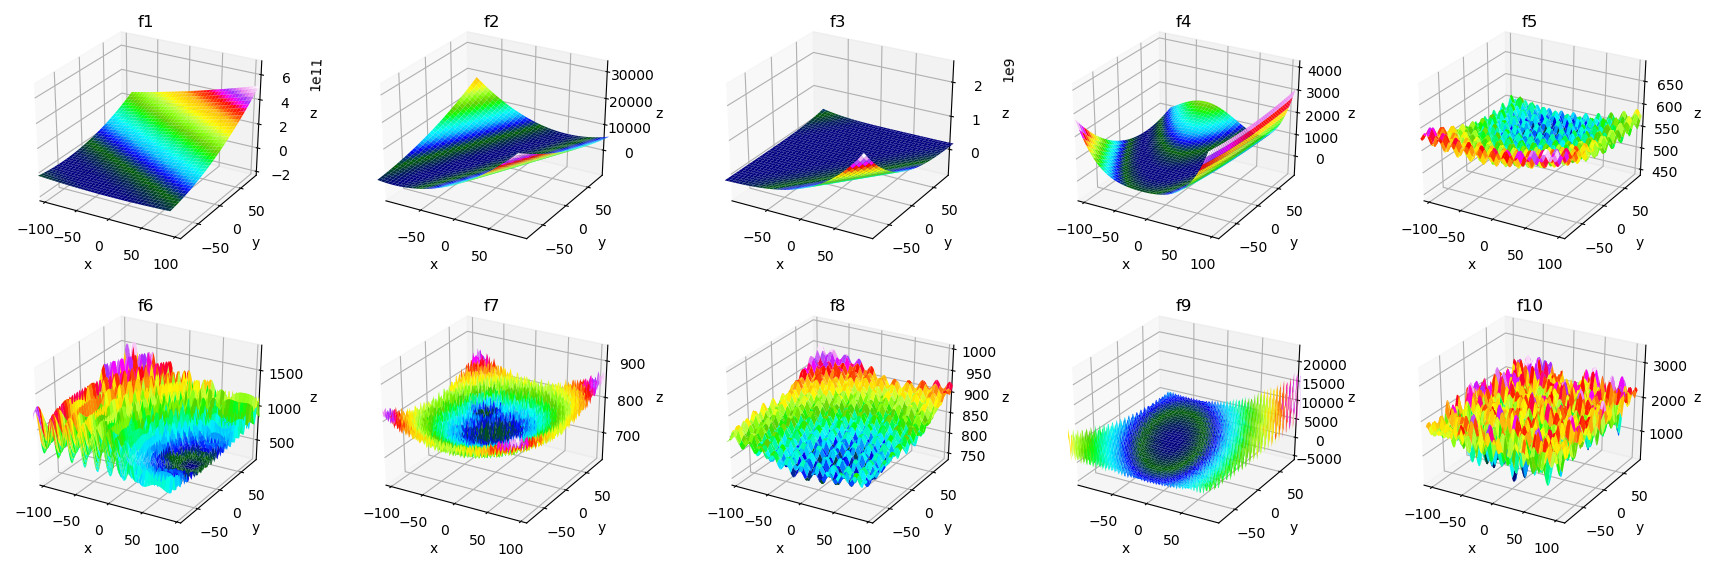
\includegraphics[width=1\linewidth]{img/cec}
	\caption{Superficies ploteadas de las 10 primeras funciones para dos dimensiones \cite{plot}}
	\label{fig:cec}
\end{figure}